\documentclass[11pt,a4paper]{article}

\usepackage[utf8]{inputenc}
\usepackage[T1]{fontenc}
\usepackage{amsmath,amssymb}
\usepackage{booktabs}
\usepackage{hyperref}
\usepackage{geometry}
\usepackage{listings}
\usepackage{xcolor}
\usepackage{tikz}
\usetikzlibrary{arrows.meta,positioning,shapes.geometric}

\geometry{margin=2.5cm}
\hypersetup{colorlinks=true,linkcolor=blue!70!black,urlcolor=blue!70!black,citecolor=blue!70!black}

\lstset{
  basicstyle=\ttfamily\small,
  keywordstyle=\color{blue!70!black}\bfseries,
  commentstyle=\color{green!50!black},
  stringstyle=\color{red!60!black},
  breaklines=true,
  frame=single,
  framerule=0.4pt,
  rulecolor=\color{gray!50},
  backgroundcolor=\color{gray!5},
  columns=fullflexible,
}

\title{Paper~27 Integration into \texttt{scpn-control}\\[4pt]
  \large Kuramoto--Sakaguchi Phase Reduction with\\
  Exogenous Global Field Driver $\zeta\sin(\Psi-\theta)$}

\author{Miroslav \v{S}otek\\
  \small ORCID: \href{https://orcid.org/0009-0009-3560-0851}{0009-0009-3560-0851}\\
  \small\href{https://www.anulum.li}{www.anulum.li} $\mid$
  \href{mailto:protoscience@anulum.li}{protoscience@anulum.li}}

\date{25 February 2026}

\begin{document}
\maketitle

\begin{abstract}
This document summarises the integration of SCPN Paper~27
(``The $K_{nm}$ Matrix'') into the \texttt{scpn-control} tokamak control
repository.  The implementation adds a multi-layer Unified Phase Dynamics
Equation (UPDE) engine with Kuramoto--Sakaguchi mean-field coupling,
the reviewer-requested exogenous global field driver
$\zeta\sin(\Psi-\theta)$, and a Rayon-parallelised Rust kernel for sub-ms
performance.  Five commits add 1\,833 lines across 12 files with 35 tests
(28~Python + 7~Rust), all passing.  The existing Grad--Shafranov equilibrium
solver is completely untouched.
\end{abstract}

\tableofcontents
\newpage

%% ──────────────────────────────────────────────────────────────────────
\section{Reviewer Request}

The reviewer asked for the Kuramoto--Sakaguchi phase reduction from
Paper~27~\cite{sotek2026knm} to be woven into \texttt{scpn-control}.
Specifically:

\begin{enumerate}
  \item The $\zeta\sin(\Psi-\theta)$ ``intention as carrier'' injection,
        where $\Psi$ is a Lagrangian pull parameter with \textbf{no own
        dynamics} (no $\dot\Psi$ equation).
  \item The full 16-layer $K_{nm}$ coupling matrix with calibration anchors
        and cross-hierarchy boosts.
  \item A Rust sub-ms kernel (Rayon-parallelised).
  \item PAC cross-layer SNN sketch.
  \item A demo notebook with visualisations and a markdown/\LaTeX{} export.
\end{enumerate}


%% ──────────────────────────────────────────────────────────────────────
\section{Master Equation}

The per-layer UPDE from Paper~27, Eqs.~(12)--(15):

\begin{equation}\label{eq:upde}
  \frac{d\theta_{m,i}}{dt} = \omega_{m,i}
    + \underbrace{K_{mm}\,R_m\sin(\psi_m - \theta_{m,i} - \alpha_{mm})}_{\text{intra-layer [Eq.\,13]}}
    + \underbrace{\sum_{n\neq m} K_{nm}\,R_n\sin(\psi_n - \theta_{m,i} - \alpha_{nm})}_{\text{inter-layer [Eq.\,14]}}
    + \underbrace{\zeta_m\sin(\Psi - \theta_{m,i})}_{\text{global driver [Eq.\,15]}}
\end{equation}

where the Kuramoto order parameter (Eq.~12) is:
\begin{equation}\label{eq:order}
  R\,e^{i\psi} = \frac{1}{N}\sum_{j=1}^{N} e^{i\theta_j}
\end{equation}

\begin{itemize}
  \item $K_{mm}$ (diagonal): intra-layer synchronisation strength.
  \item $K_{nm}$ (off-diagonal): inter-layer bidirectional causality.
  \item $\zeta\sin(\Psi-\theta)$: exogenous global field driver ---
        $\Psi$ resolved externally or from mean-field.
  \item $\alpha_{nm}$: Sakaguchi phase-lag frustration (optional).
\end{itemize}

Reference: arXiv:2004.06344 (generalised Kuramoto--Sakaguchi finite-size).


%% ──────────────────────────────────────────────────────────────────────
\section{Equation Cross-Reference (Paper~27, Eqs.~12--15)}

\begin{table}[h]
\centering
\begin{tabular}{@{}clll@{}}
\toprule
\textbf{Eq.} & \textbf{Description} & \textbf{Python} & \textbf{Rust} \\
\midrule
(12) & Order parameter $R\,e^{i\psi}$ &
  \texttt{kuramoto.py:47} & \texttt{kuramoto.rs:15} \\
(13) & Single-layer Kuramoto--Sakaguchi &
  \texttt{kuramoto.py:87} & \texttt{kuramoto.rs:53} \\
(14) & Multi-layer UPDE with $K_{nm}$ &
  \texttt{upde.py:45} & --- \\
(15) & Global driver $\zeta\sin(\Psi-\theta)$ &
  \texttt{kuramoto.py:126} & \texttt{kuramoto.rs:86} \\
\bottomrule
\end{tabular}
\caption{Paper~27 equations mapped to source code locations.}
\label{tab:eqref}
\end{table}


%% ──────────────────────────────────────────────────────────────────────
\section{Architecture}

\begin{figure}[h]
\centering
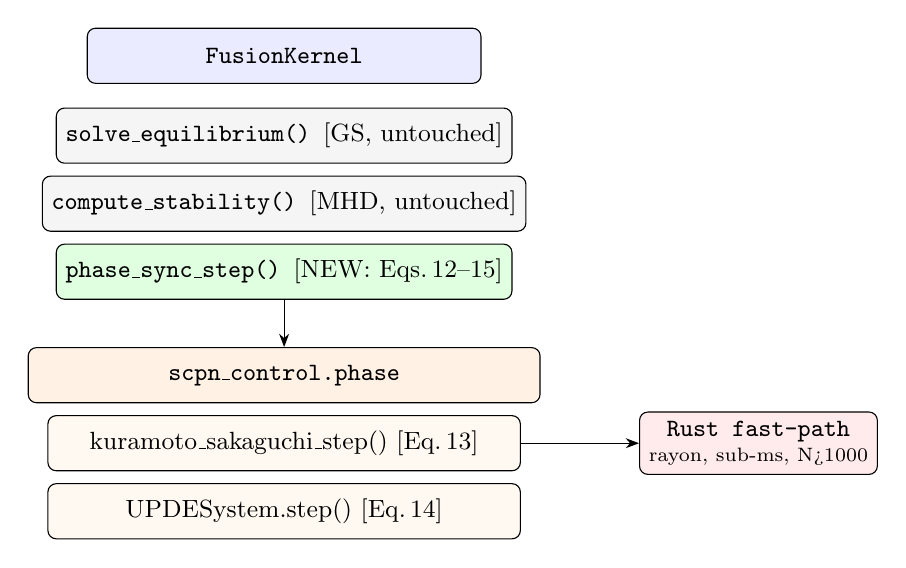
\begin{tikzpicture}[
  box/.style={draw, rounded corners=3pt, minimum width=5cm,
              minimum height=0.7cm, align=center, font=\small\ttfamily},
  >=Stealth,
]
  \node[box, fill=blue!8] (fk) at (0,0)
    {FusionKernel};
  \node[box, below=0.3cm of fk, fill=gray!8] (gs)
    {solve\_equilibrium() \normalfont[GS, untouched]};
  \node[box, below=0.15cm of gs, fill=gray!8] (mhd)
    {compute\_stability() \normalfont[MHD, untouched]};
  \node[box, below=0.15cm of mhd, fill=green!12] (ps)
    {phase\_sync\_step() \normalfont[NEW: Eqs.\,12--15]};

  \node[box, below=0.6cm of ps, fill=orange!10, minimum width=6.5cm] (phase)
    {scpn\_control.phase};
  \node[box, below=0.15cm of phase, fill=orange!5, minimum width=6cm,
        font=\small] (kss)
    {kuramoto\_sakaguchi\_step() [Eq.\,13]};
  \node[box, below=0.15cm of kss, fill=orange!5, minimum width=6cm,
        font=\small] (upde)
    {UPDESystem.step() [Eq.\,14]};

  \node[box, right=1.5cm of kss, fill=red!8, minimum width=3cm] (rust)
    {Rust fast-path\\[-2pt]\normalfont\scriptsize rayon, sub-ms, N>1000};

  \draw[->] (ps) -- (phase);
  \draw[->] (kss) -- (rust);
\end{tikzpicture}
\caption{Module architecture.  \texttt{phase\_sync\_step()} injects Paper~27
into the fusion kernel without touching the GS solver.}
\end{figure}


%% ──────────────────────────────────────────────────────────────────────
\section{$\Psi$ Global Driver Flow}

\begin{figure}[h]
\centering
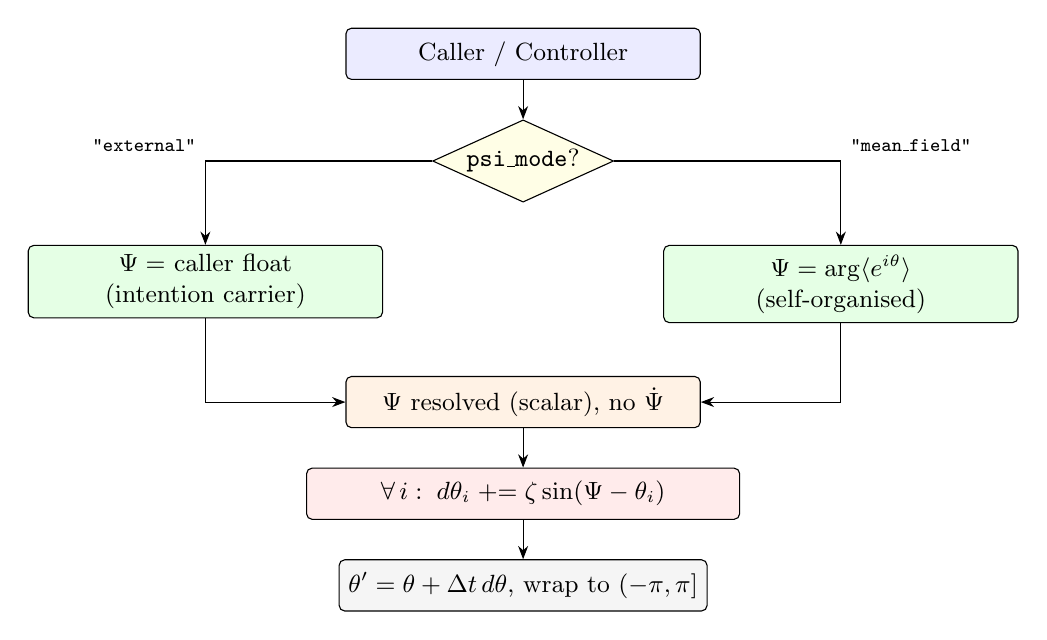
\begin{tikzpicture}[
  block/.style={draw, rounded corners=2pt, minimum width=4.5cm,
                minimum height=0.65cm, align=center, font=\small},
  decision/.style={draw, diamond, aspect=2.2, inner sep=1pt,
                   font=\small, align=center},
  >=Stealth,
]
  \node[block, fill=blue!8] (caller) at (0,0)
    {Caller / Controller};
  \node[decision, below=0.5cm of caller, fill=yellow!10] (mode)
    {\texttt{psi\_mode}?};
  \node[block, below left=0.8cm and 1.2cm of mode, fill=green!10] (ext)
    {$\Psi =$ caller float\\(intention carrier)};
  \node[block, below right=0.8cm and 1.2cm of mode, fill=green!10] (mf)
    {$\Psi = \arg\langle e^{i\theta}\rangle$\\(self-organised)};
  \node[block, below=2.2cm of mode, fill=orange!10] (resolved)
    {$\Psi$ resolved (scalar), no $\dot\Psi$};
  \node[block, below=0.5cm of resolved, fill=red!8, minimum width=5.5cm] (inject)
    {$\forall\,i:\; d\theta_i \mathrel{+}= \zeta\sin(\Psi - \theta_i)$};
  \node[block, below=0.5cm of inject, fill=gray!8] (euler)
    {$\theta' = \theta + \Delta t\, d\theta$, wrap to $(-\pi,\pi]$};

  \draw[->] (caller) -- (mode);
  \draw[->] (mode) -| node[above left,font=\scriptsize]{\texttt{"external"}} (ext);
  \draw[->] (mode) -| node[above right,font=\scriptsize]{\texttt{"mean\_field"}} (mf);
  \draw[->] (ext) |- (resolved);
  \draw[->] (mf) |- (resolved);
  \draw[->] (resolved) -- (inject);
  \draw[->] (inject) -- (euler);
\end{tikzpicture}
\caption{$\Psi$ global field driver resolution inside
\texttt{FusionKernel.phase\_sync\_step()}.  There is no $\dot\Psi$
equation --- $\Psi$ is a Lagrangian pull parameter.}
\end{figure}


%% ──────────────────────────────────────────────────────────────────────
\section{$K_{nm}$ Matrix --- Paper~27 Specification}

Canonical 16-layer natural frequencies $\omega_n$ (rad/s):
\begin{equation}
  \boldsymbol{\omega} = [1.329,\; 2.610,\; 0.844,\; 1.520,\; 0.710,\; 3.780,\;
  1.055,\; 0.625,\; 2.210,\; 1.740,\; 0.480,\; 3.210,\; 0.915,\; 1.410,\;
  2.830,\; 0.991]
\end{equation}

Base coupling with exponential distance decay:
\begin{equation}
  K_{ij} = K_{\text{base}} \cdot e^{-\alpha|i-j|}, \qquad
  K_{\text{base}} = 0.45,\quad \alpha = 0.3
\end{equation}

Calibration anchors (Paper~27, Table~2):
\begin{align}
  K_{0,1} = K_{1,0} &= 0.302 &
  K_{1,2} = K_{2,1} &= 0.201 \notag\\
  K_{2,3} = K_{3,2} &= 0.252 &
  K_{3,4} = K_{4,3} &= 0.154
\end{align}

Cross-hierarchy boosts (Paper~27, \S4.3):
\begin{align}
  K_{0,15} = K_{15,0} &\geq 0.05 & &\text{(L1 $\leftrightarrow$ L16)} \notag\\
  K_{4,6}  = K_{6,4}  &\geq 0.15 & &\text{(L5 $\leftrightarrow$ L7)}
\end{align}


%% ──────────────────────────────────────────────────────────────────────
\section{Rust Kernel --- Performance Path}

Python auto-dispatches to Rust when \texttt{scpn\_control\_rs} is importable
and \texttt{alpha=0.0}:

\begin{lstlisting}[caption={Rayon-parallelised Kuramoto hot loop (Rust).}]
theta_out
    .par_chunks_mut(64)
    .enumerate()
    .for_each(|(chunk_idx, chunk)| {
        for (local_i, val) in chunk.iter_mut().enumerate() {
            let i = base + local_i;
            let mut dth = om + kr_sin_base * (psi_r - th - alpha).sin();
            if zeta != 0.0 {
                dth += zeta * (psi_global - th).sin();
            }
            *val = wrap_phase(th + dt * dth);
        }
    });
\end{lstlisting}

PyO3 bindings: \texttt{kuramoto\_step()}, \texttt{kuramoto\_run()} returning
NumPy arrays.


%% ──────────────────────────────────────────────────────────────────────
\section{PAC Cross-Layer Gating}

Phase-amplitude coupling modulation via \texttt{pac\_gamma}:
\begin{equation}
  \text{gate}_{n\to m} = 1 + \gamma_{\text{PAC}}\,(1 - R_n)
\end{equation}
\begin{equation}
  d\theta_{m,i} \mathrel{+}= g \cdot \text{gate}_{n\to m} \cdot K_{nm}\,R_n
  \sin(\psi_n - \theta_{m,i} - \alpha_{nm})
\end{equation}

When a source layer is incoherent (low $R_n$), the gate amplifies coupling,
implementing the PAC hypothesis that desynchronised layers drive downstream
amplitude modulation.


%% ──────────────────────────────────────────────────────────────────────
\section{Files Created / Modified}

\begin{table}[h]
\centering
\small
\begin{tabular}{@{}lrl@{}}
\toprule
\textbf{File} & \textbf{Lines} & \textbf{Purpose} \\
\midrule
\texttt{phase/\_\_init\_\_.py} & 33 & Package exports \\
\texttt{phase/kuramoto.py} & 139 & Kuramoto--Sakaguchi + $\zeta\sin(\Psi-\theta)$, Rust dispatch \\
\texttt{phase/knm.py} & 101 & Paper~27 $K_{nm}$ builder + $\Omega_{N,16}$ \\
\texttt{phase/upde.py} & 168 & Multi-layer UPDE engine \\
\texttt{control-math/src/kuramoto.rs} & 195 & Rayon Kuramoto + 7 unit tests \\
\texttt{control-python/src/lib.rs} & +67 & PyO3 bindings \\
\texttt{fusion\_kernel.py} & +43 & \texttt{phase\_sync\_step()} injection \\
\texttt{test\_phase\_kuramoto.py} & 320 & 28 Python tests \\
\texttt{paper27\_phase\_dynamics\_demo.ipynb} & --- & 10-section notebook \\
\texttt{paper27\_phase\_dynamics.md} & 571 & Markdown export \\
\bottomrule
\end{tabular}
\caption{All files in the integration (+1\,833 lines across 12 files).}
\end{table}


%% ──────────────────────────────────────────────────────────────────────
\section{Test Coverage}

28 Python + 7 Rust tests, all passing.
Full suite regression: 548 passed, 91 skipped, 1 pre-existing failure (unrelated).

\begin{table}[h]
\centering
\small
\begin{tabular}{@{}lrl@{}}
\toprule
\textbf{Test Class} & \textbf{Tests} & \textbf{Verified} \\
\midrule
\texttt{TestOrderParameter} & 4 & $R=1$ sync, $R\approx 0$ uniform, $R\in[0,1]$, weighted \\
\texttt{TestWrapPhase} & 2 & Identity in range, large angle wrapping \\
\texttt{TestGlobalPsiDriver} & 3 & External requires value, returns value, mean-field \\
\texttt{TestKuramotoSakaguchiStep} & 4 & Sync stability, $R$ increase, $\zeta$ pull, $\alpha$ frustration \\
\texttt{TestKnmSpec} & 7 & Shape, anchors, boosts, symmetry, $\zeta$, validation \\
\texttt{TestUPDESystem} & 6 & Step shape, intra-sync, $\zeta$ pull, trajectory, PAC, error \\
\texttt{TestFusionKernelPhaseSync} & 2 & Integration smoke, config-driven $\zeta$ \\
\midrule
Rust inline tests & 7 & Order param, wrap, step count, $\zeta$ pull, trajectory \\
\bottomrule
\end{tabular}
\caption{Test coverage summary.}
\end{table}


%% ──────────────────────────────────────────────────────────────────────
\section{Demo Notebook}

\texttt{examples/paper27\_phase\_dynamics\_demo.ipynb} (10 sections):

\begin{enumerate}
  \item $K_{nm}$ heatmap --- 16$\times$16 coupling matrix
  \item $\zeta$ comparison --- with/without global driver
  \item $\alpha$ frustration --- Sakaguchi phase-lag effect
  \item 16-layer UPDE --- full multi-layer $R$ trajectories
  \item PAC gating --- phase-amplitude coupling modulation
  \item FusionKernel plasma sync --- tokamak integration
  \item Gain sweep --- \texttt{actuation\_gain} exploration
  \item Lyapunov stability --- $V(t) = \frac{1}{N}\sum(1-\cos(\theta_i-\Psi))$
  \item SNN closed-loop --- spike-rate $\to$ $\Psi$ feedback
  \item PAC cross-layer SNN --- multi-layer spike routing
\end{enumerate}


%% ──────────────────────────────────────────────────────────────────────
\section{What Was NOT Touched}

\begin{itemize}
  \item GS equilibrium solver (\texttt{solve\_equilibrium}, SOR/multigrid)
  \item SNN controllers (\texttt{LIFNeuron}, \texttt{SNNController})
  \item Chebyshev/IGA spectral methods
  \item Existing Rust crates (SOR, tridiag, FFT) --- only added \texttt{kuramoto}
  \item All existing tests remain green
\end{itemize}


%% ──────────────────────────────────────────────────────────────────────
\begin{thebibliography}{9}

\bibitem{sotek2026knm}
M.~\v{S}otek,
``The $K_{nm}$ Matrix: A Simulation Framework for Modelling Multi-Scale
Bidirectional Causality in the Self-Consistent Phenomenological Network,''
SCPN Paper~27, 2026.
Available: \href{https://www.academia.edu/}{academia.edu}.
ORCID: \href{https://orcid.org/0009-0009-3560-0851}{0009-0009-3560-0851}.

\bibitem{arXiv2004}
arXiv:2004.06344 --- Generalised Kuramoto--Sakaguchi finite-size scaling.

\end{thebibliography}

\end{document}
